\documentclass[12pt,a4paper]{article}
\usepackage{solutions-en}
\usepackage{float}
\usepackage[normalem]{ulem}
\usepackage[all]{xy}
\CompileMatrices

\title{Homework of 10.12\\Differential geometry}
\author{Gleb Minaev @ 204 (20.Б04-мкн)}
\date{}

\newcommand{\const}{\mathrm{const}}
\newcommand{\R}{\mathrm{R}}

\begin{document}
    \maketitle

    \begin{problem}{60}
        We know that $|\gamma(t + \delta) - \gamma(t)|$ depends on only $\delta$; then let $l(\delta) := |\gamma(t + \delta) - \gamma(t)|$. So for any $t \in (a; b)$
        \[
            |\gamma'(t)|
            = \left|\lim_{\delta \to 0} \frac{\gamma(t+\delta) + \gamma(t)}{\delta}\right|
            = \lim_{\delta \to 0} \frac{|\gamma(t+\delta) + \gamma(t)|}{|\delta|}
            = \lim_{\delta \to 0} \frac{l(\delta)}{|\delta|}
        \]
        does not depend on $t$, i.e. $|\gamma'| = \const$ on $[a; b]$. Also $|\gamma(t + \delta) - \gamma(t)|$ being a constant function of $t$ for any fixed $\delta$ means that
        \[(\gamma(t + \delta) - \gamma(t)) \cdot (\gamma'(t + \delta) - \gamma'(t)) = 0,\]
        i.e. $\gamma(t + \delta) - \gamma(t)$ and $\gamma'(t + \delta) - \gamma'(t)$ are perpendicular (or one of them is a zero vector).

        If $|\gamma'| = 0$, then $\gamma' = 0$ and $\gamma = \const$. Hence in that case problem is obvious. Then let's consider case $|\gamma'| > 0$.

        \begin{lemma}
            Let $p, q, r \in [a; b]$ be three different points such that $\gamma(p)$, $\gamma(q)$ and $\gamma(r)$ are different in pairs and lie on some circle $\omega$ (so are not collinear). Let $O$ be a center of $\omega$ and $R_\varphi$ is operator of rotation (of vector) by $\varphi$ counterclockwise. Then $\gamma'(p) = \gamma'(q) = \gamma'(r)$ or there is $\lambda \in \RR$ such that
            \[
                \gamma'(p) = \lambda \R_{\pi/2}(\gamma(p) - O),
                \qquad
                \gamma'(q) = \lambda \R_{\pi/2}(\gamma(q) - O),
                \qquad
                \gamma'(r) = \lambda \R_{\pi/2}(\gamma(r) - O).
            \]
        \end{lemma}

        \begin{proof}
            Let's name $P := \gamma(p)$, $Q := \gamma(q)$ and $R := \gamma(r)$, $v_p := \R_{-\pi/2}(\gamma'(p))$, $v_q := \R_{-\pi/2}(\gamma'(q))$ and $v_r := \R_{-\pi/2}(\gamma'(r))$. Then $v_p - v_q$ is (zero vector or) parallel to $\overline{PQ}$; and the same goes for $p$ and $r$, $q$ and $r$. Let $\sigma$ be a circle with center $R - v_r$ and goes through $R$, and $P'$, $Q'$ be secondary intersection of $\sigma$ with $\overline{RP}$ and $\overline{RQ}$.
            \begin{figure}[H]
                \centering
                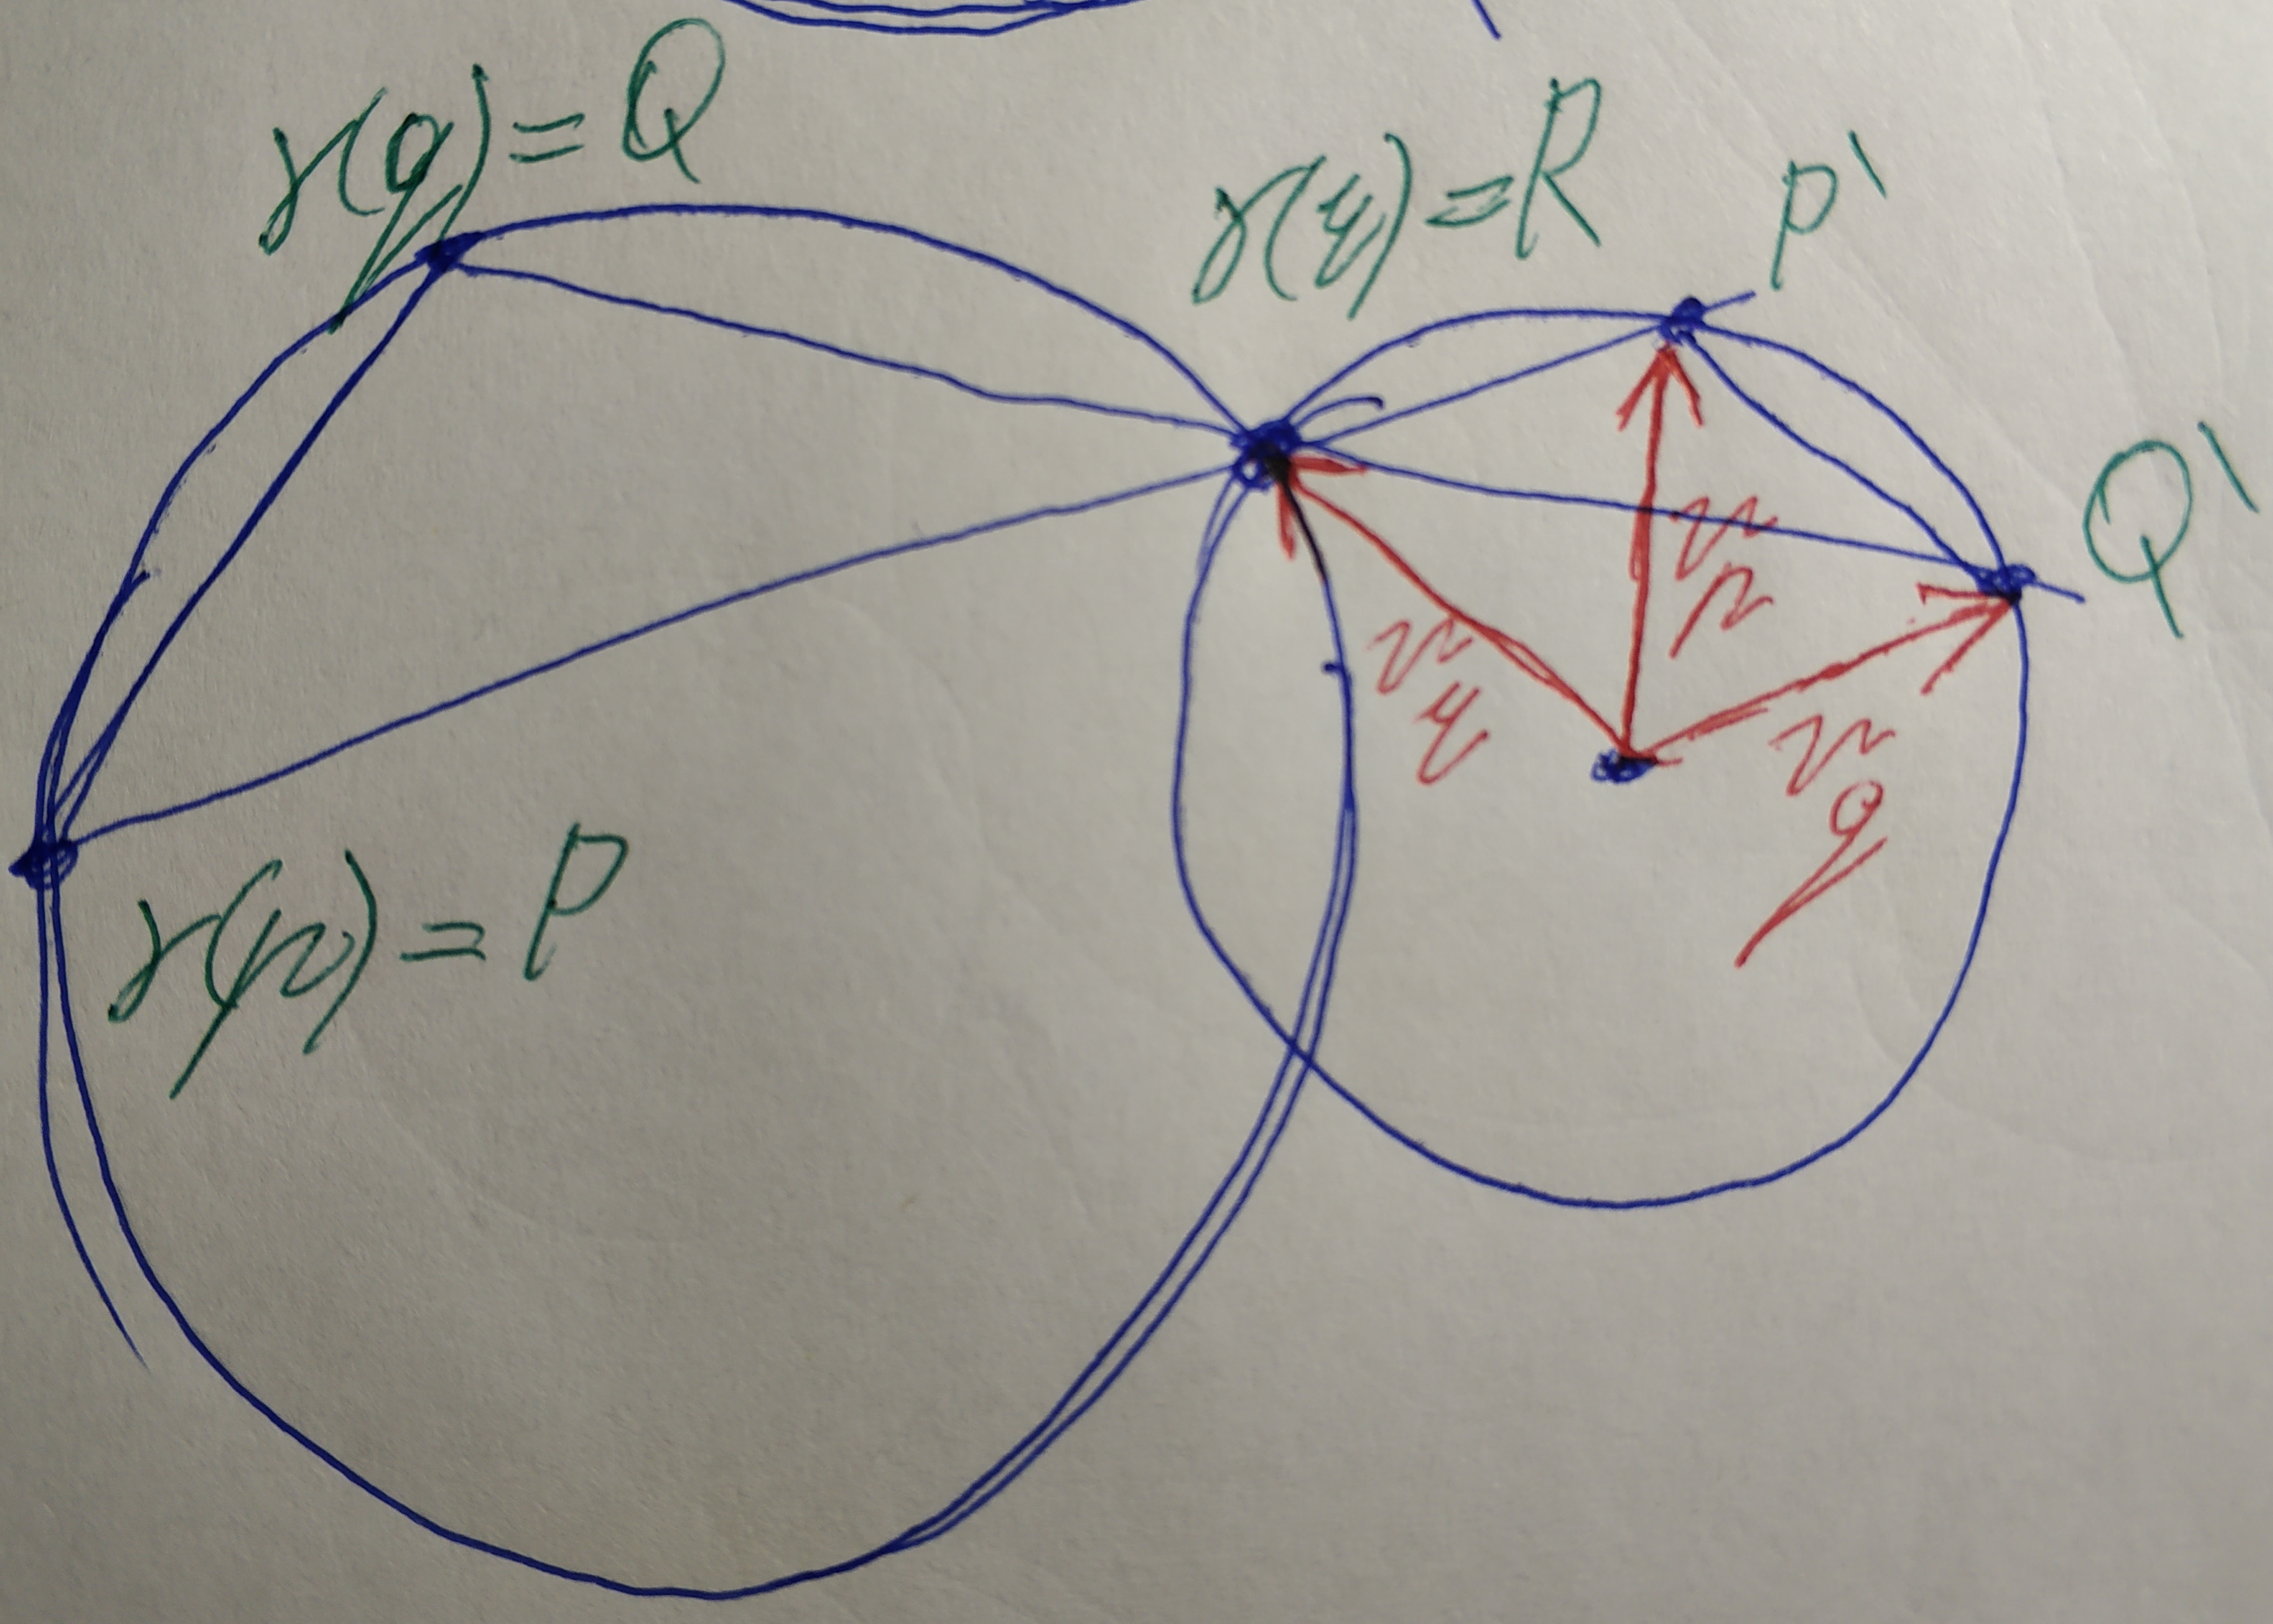
\includegraphics[height=5cm]{DG-HW-006-1.jpg}
            \end{figure}
            Let $O'$ be center of $\sigma$. $v_p - v_r \parallel \overline{PR}$, so $R - v_r + v_p \in \overline{PR}$, i.e. $O' + v_p$ is $R$ or $P'$; similarly $O' + v_q \in \{R; Q'\}$.
            
            If $v_p = v_r$ then $v_p - v_q = v_r - v_q$ is parallel to both $\overline{PQ}$ and $\overline{RQ}$ (that are not parallel, so $v_q - v_r = 0$, $v_q = v_r$. Similarly if $v_q = v_r$ then $v_p = v_r$. Then let's consider case $v_p = P' - O'$ and $v_q = Q' - O'$.

            Then $v_p - v_q = P' - Q'$ is parallel to $\overline{PQ}$. So homotety with center $R$ and coefficient $\lambda := \overrightarrow{RP}/\overrightarrow{RP'}$ maps $R$ to $R$, $P$ to $P'$, line $\overline{RQ'}$ to itself, $\overline{P'Q'}$ to parallel line through $P$ that is $\overline{PQ}$, so $Q'$ to $Q$. Hence it maps $v_p$, $v_q$ and $v_r$ to $P - O$, $Q - O$ and $R - O$. It means
            \[\gamma'(p) = \R_{\pi/2}(v_p) = \R_{\pi/2}(\lambda(\gamma(p) - O)) = \lambda \R_{\pi/2}(\gamma(p) - O);\]
            the same goes to $q$ and $r$.
        \end{proof}

        \begin{corollary}
            If $\gamma(p)$, $\gamma(q)$ and $\gamma(r)$ are not collinear and $\gamma'(p)$, $\gamma'(q)$ and $\gamma'(r)$ are different, then $\gamma'(p)$, $\gamma'(q)$ and $\gamma'(r)$ constructed from $\gamma(p)$, $\gamma(q)$ and $\gamma(r)$ respectievly are tangent to circumcircle of $\gamma(p)$, $\gamma(q)$ and $\gamma(r)$, have the same length and are oriented in the same direction along the circumcircle.
        \end{corollary}

        \begin{corollary}
            If $\gamma(p) \neq \gamma(q)$ and $\gamma'(p) \neq \gamma'(q)$ then for every $r$ if $\gamma(r) \notin \overline{\gamma(p) \gamma(q)}$ then $\gamma(r)$ is lying on circle through $\gamma(p)$ and $\gamma(q)$ that is tangent to $\gamma'(p)$ constructed from $\gamma(p)$. 
        \end{corollary}

        So if there are two arguments $p, q \in [a; b]$ such that $\gamma(p) \neq \gamma(q)$ and $\gamma'(p) \neq \gamma'(q)$, then all points of $\gamma$ are lying in union of a circle and a line that have intersection $\{\gamma(p); \gamma(q)\}$. But obviously because of smoothness of $\gamma$ it can not go from the circle to the line (there will be a breaking in point where $\gamma$ will change its trajectory from the circle to the line or vice versa). Then $\gamma$ is lying on some line or some circle.

        Then the remaining case is where for any $p, q \in [a; b]$ $\gamma(p) = \gamma(q)$ or $\gamma'(p) = \gamma'(q)$. Then if $\gamma = \const$ the problem is obvious; otherwise there are $p, q \in [a; b]$ such that $\gamma(p) \neq \gamma(q)$. Then $\gamma'(p) = \gamma'(q)$. So for any $r \in [a; b]$ $\gamma(r) \neq \gamma(p)$ or $\gamma(r) \neq \gamma(q)$, so then $\gamma'(r) = \gamma'(p) = \gamma'(q)$. Hence $\gamma' = \const$, so $\gamma = A + tv$ that is lying on a line through $A$ and is parallel to $v$.
    \end{problem}
\end{document}